\chapter{Konzept}
\section{Allgemeines}
\subsection{Zweck}

\section{Ausgangslage}
Der Abschnitt hier basiert auf dem vorangehenden Entscheid bei der Auswahl des Rich Client Frameworks. Aus den im Abschnitt \titleref{rcp_entscheid} beschriebenen und nachvollziehbaren Gründen wird zur Implementation des Garbage Collection Log Analyzers die Eclipse Rich Client Plattform in der Version 3.x\footnote{die aktuelle Version ist 3.7 (stand: 31.8.2011)} genommen. Die in der Anforderungsanalyse allgemein definierten Anforderungen werden nun spezifisch auf diese Plattform konzipiert, für die einzelnen Thematiken werden nun auch die Begrifflichkeiten innerhalb Eclipse verwendet.


\section{Umgebung}
\subsection{Build-Automation}
Die Automatisierung des Software-Builds ist hinsichtlich der Integration in ein Continuous Integration System Voraussetzung. Es hat zusätzlich aber andere Vorteile:
\begin{itemize}
	\item Tasks wie das Kompilieren, die Packetierung und das Deployment der Software müssen nicht mehr manuell gemacht werden.
	\item Zur Verhinderung von Regression und entsprechend zur Gewährleistung der Qualität können vor jedem Release automatisch die Tests durchgeführt werden.
\end{itemize}


Als Werkzeug zum automatisierten Build der Software wird Maven Tycho\footnote{Im Bereich der Eclipse Rich Client Entwicklung kann entweder PDE Build, ein auf Apache Ant basiertes Build-System für Eclipse RCP Applikationen\cite{vogelZapfPdeBuild} oder die Maven-Integration Tycho (http://tycho.sonatype.org) verwendet werden.} verwendet. Um Tycho führt mittlerweile kein Weg drum herum, es hat im Vergleich zum PDE Build einige Vorteile:
\begin{itemize}
	\item Maven Builds lassen sich ohne grossen Aufwand in Continuous Integration Systeme integrieren.
	\item Maven hat eine gute Integration in alle gängigen Entwicklungsumgebungen\footnote{Projekt-Dateien müssen nicht mehr in die Versionskontrolle eingecheckt werden.} und ist sehr verbreitet
\end{itemize}

\subsection{Continous Integration}
Als Continuous Integration Server wird Jenkins\footnote{http://jenkins-ci.org - Jenkins ist der ehemalige Hudson CI Server, welcher nach dem Kauf von Sun durch Oracle als Branch entstanden ist.} verwendet. Jenkins bringt nebst seiner Benutzerfreundlichkeit als Build Server einige zum Projekt nötigen Voraussetzungen mit:
\begin{itemize}
	\item Jenkins ist für alle denkbaren Betriebssysteme vorhanden.
	\item Jenkins ist kompatibel mit allen gängigen Systemen zur Versionskontrolle: Git, Subversion, CVS, etc.
	\item Maven-Projekte lassen sich ohne grossen Aufwand als Build-Projekte konfigurieren.
\end{itemize}

\subsection{Versionskontrolle}
Zur Versionskontrolle kommen mehrere Werkzeuge in Frage. Da Git\footnote{http://git-scm.com} in einigen Bereichen besser ist als Subversion, CVS und zusätzlich mit Github\footnote{http://github.com} ein darauf basierendes freies Repository verfügbar ist, wird Git verwendet.
\subsection{Issue Tracker}
Als Issue Tracker wird Jira verwendet. Es handelt sich zwar im Gegensatz zu Bugzilla um eine kostenpflichtige Software, die geringen kosten lohnen sich aber alle weil. 

\section{Installation der Software}\label{installation}
Auf der Eclipse Plattform können Funktionalitäten auf unterschiedliche Arten verteilt werden. Es handelt sich in der Regel aber um Java-Archive (Jars) die mit gewissen Meta-Informationen versehen sind. Diese Archive können sich sowohl lokal auf dem Dateisystem befinden oder via eine Update-Seite, wobei es sich um den wesentlich effizienteren Weg handelt, bereitgestellt werden. Die Funktionalität zu diesem Prozess stellt das Eclipse Framework bereits zur Verfügung: Update-Seiten\footnote{Update-Seiten werden ebenfalls als Eclipse-Projekte definiert} beinhalten Kategorien mit Features. Ein Feature ist wiederum eine wohldefinierte Software-Komponente bestehend aus unterschiedlichen Plugins - bei diesen handelt es sich um die kleinst mögliche Komponente die aus der Programmlogik und der Schnittstellendefinition\footnote{Plugins definieren die Schnittstelle durch Abhängigkeiten, Exportierte Packete, Importierte Packete und Extension-Points.} besteht.

Die Update-Seite für diese Software wird folgendermassen aufgebaut:
\begin{itemize}
	\item Garbage Collection Log Analysis (Kategorie)
		\begin{itemize}
			\item Core (Feature)
			\item JRockit Extension (Feature)
		\end{itemize}
\end{itemize}
Der Vorteil dieser Struktur ist, dass man nachträglich noch zusätzliche Extensions hinzufügen kann.


\section{Architektur}
\subsection{Basiskomponenten}
Wie im Abschnitt \titleref{installation} erläutert, besteht die Software aus zwei getrennten Features. Das Core-Feature ist verantwortlich für den gesamten Import-Prozess (Import-Wizard, Leseprozess der Log-Datei, Anzeige der Menus, etc.). Die JRockit Extension ist eine wird benötigt, um überhaupt den Inhalt der Log Dateien zu parsen, ein adäquates Domänenmodell zu erstellen und die Charts/Reports dafür anzuzeigen. Diese Aufteilung hat zum Zweck, dass die Software mit anderen Log-Formaten erweitert werden kann.
 \begin{figure}[H]
  	\centering
        	\caption{Architektur: Komponentendiagramm}
    	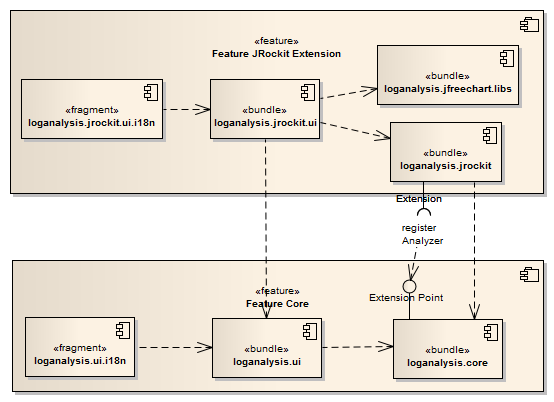
\includegraphics[width=15cm]{images/architektur_komponenten_uebersicht}
\end{figure}

Das Core Feature besteht aus dem Modul User Interface (``loganalysis.core.ui'') und einer von JFace und SWT\footnote{JFace und SWT wird in Eclipse als Library für den Presentation Layer verwendet} unabhängigen Teil (``loganalysis.core''). Startet der Anwender einen Import einer Garbage Collection Datei, werden durch das Core-Feature alle registrierten Extensions abgefragt, ob sie den Inhalt dieser Datei verstehen. Sobald dies zutrifft, wird das Parsing und die Anzeige des Reports, Charts an diese Extension delegiert. Im Eclipse Framework passiert diese Registrierung über das Prinzip der Extension-Points.

\subsection{Weitere Bundles}
Zusätzlich zu den behandelten Plugins wurden noch einige nicht erwähnt:

\begin{itemize}
	\item Feature Bundles
		\begin{itemize}
			\item loganalysis.feature
			\item loganalysis.jrockit.feature
		\end{itemize}
	\item Thirdparty Bibliotheken
		\begin{itemize}
			\item  loganalysis.jfreechart.libs (JFreeChart Library)
		\end{itemize}
	\item Diverses
		\begin{itemize}
			\item  loganalysis.targetplatform (beinhaltet die Target-Plattform)
			\item loganalysis.updatesite (definiert und generiert die Update-Seite)
		\end{itemize}
\end{itemize}




